\documentclass[../MaxHughesThesis.tex]{subfiles}

\begin{document}

For a potential beta energy spectrum shape measurement, several criteria for a nucleus are needed.
The first is that the nucleus and the decay mode must be available in sufficient quantities that a proper decay spectrum shape can be measured.
This means that the nucleus needs to be relatively close to stability.
The decay mode needs to be clean.
If there are several competing decay modes of similar strength, the shape of the beta decay spectrum gets complicated.
The same thing happens if there are several gamma rays in the decay. 
Having one gamma ray is useful, as a coincidence measurement can be used to exclude much of any background in the measurement.
In order to get a useful theoretical interpretation of the measurement of the Fierz term, a purely Fermi or Gamow-Teller transition is needed.
An allowed Gamow-Teller transition gives sensitivity to tensor couplings. 
A nucleus that fulfills these criteria is $^{20}$F. 
 
\section{$^{20}$F Decay Characteristics}

The decay scheme is given in figure \ref{fig:DecayScheme}.
As seen in the figure, $^{20}$F decays 99.99\% of the time to the first excited state of $^{20}$Ne.
This decay is very clean, as there are very few contaminants from other decay branches. 
The $2^{+}$ state seen in the decay scheme is not the isobaric analogue state to the ground state of $^{20}$F.
That state is much higher in energy.
The beta decay therefore has an isospin change of 1.
This means that the allowed Fermi matrix element is zero, and the decay is an allowed Gamow-Teller transition. 
%The forbidden transitions contribute <INSERT THEORY HERE> 
The forbidden transitions only contribute to higher order.
The half-life of $^{20}$F is about 11 seconds. 
This means waiting for the $^{20}$F to decay will take less than a minute to get good statistics.

\begin{figure}[!htb]
	\centerline{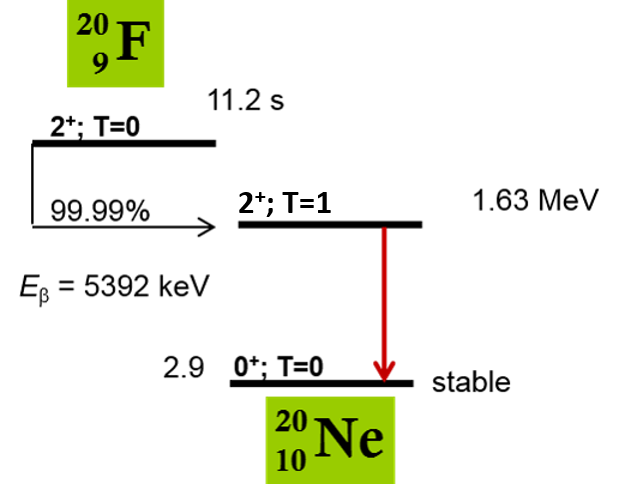
\includegraphics[width=0.5\textwidth]{20FDecayScheme_v2.png}}
	\caption{The decay scheme of $^{20}$F.}
	\label{fig:DecayScheme}
\end{figure}

The 1.6 MeV gamma ray in the transition allows for a coincidence measurement to take place.
One gamma ray does not distort the spectrum much. 
$^{20}$F is relatively close to stability, so it can be made in sufficient quantities to get high statistics.

\section{Previous Measurements in $^{20}$F Decay}

Some of the earliest measurements of $^{20}$F where $ft$ value measurements \cite{Wil70} \cite{Alb75}.
The half-lives were measured with a plastic scintillator in either case.  
These $ft$ values were compared to the mirror nucleus $^{20}$Na in order to search for second class currents in beta decay. 

Another, more recent measurement whose goal was putting limits on second class currents was done with with a polarized $^{20}$F and $^{20}$Na beam \cite{Min11}.
The technique was an alignment measurement over different energies.
The $^{20}$F was made with a polarized deuteron beam impinging on a $^{19}$F target. 
The direction of the outgoing electron was measured and recorded.
The angular distribution was measured using the beta-nuclear magnetic resonance (NMR) technique.
Plastic scintillators at the end of magnets were used to measure the direction of the electrons.
The correlations were corrected for and plotted vs energy.
The outcome of that analysis was a measurement of the various form factors that correct the beta decay spectrum shape. 
The resulting $^{20}$F energy spectrum is shown in figure \ref{fig:keispec}.
In this spectrum, there are several background contributions. 
Since this measurement  was an asymmetry measurement, the influence of the backgrounds are reduced. 
Different polarization were used to eliminate systematic effects.
Double ratios were taken to account for difference in solid angle and detector efficiency.
The threshold was taken to be 2 MeV, as below that energy, the spectrum is distorted.

\begin{figure}[!htb]
	\centerline{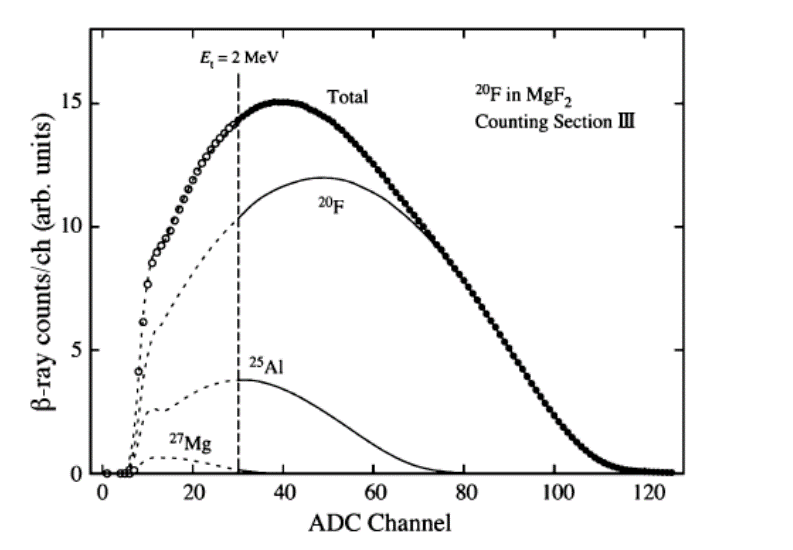
\includegraphics[width=0.75\textwidth]{Kei1120FSpectrum.png}}
	\caption{A sample beta energy spectrum using a plastic scintillator detector \cite{Min11}.}
	\label{fig:keispec}
\end{figure}

There are several important systematic effects in this measurement.
The two largest have to do with corrections for the solid angle and corrections for the 1.634 MeV gamma ray.
The corrections for the solid angle have to do with estimates of the scattering of the electrons.
This happens at the implantation target, and can happen on the walls of the spectrometer.
To counteract this effect, a veto detector was included in the detector set up. 
This veto detector was situated near the walls of the magnet, so any scattering off of the magnet could be vetoed. 
The other large systematic effect has to do with gamma rays.
Since the $^{20}$F is polarized, the direction of the emitted gamma rays is anisotropic.
The gamma rays contribute and pile-up with the detected beta spectrum in different ways.
This has to be corrected for with the detector response.
With all these effects, the second class current effects were found to be consistent with zero.   

\subsection{Shape Measurements} 

Several direct shape measurements have been made in $^{20}$F.
Two measurements with different systematic effects will be discussed.
Both of them looked for the linear term in the hardonic correction to the beta decay spectrum shape. 

A measurement of the $^{20}$F spectrum shape was done with a spectrometer \cite{Elm87}.
The goal was to measure the nuclear shape factor and get a measurement of the linear term.
This shape factor will be described further in a later chapter.
The ultimate goal was to test the conserved vector current (CVC) hypothesis. 
$^{20}$F was created with a deuteron beam on a $^{19}$F target.
The target was $^{6}$LiF on a carbon foil.
After the target was bombarded, and the $^{20}$F created, the outgoing electron went through the foil and into the spectrometer.
The spectrometer was tuned to accept a certain energy of electrons. 
Then, data on the decay of $^{20}$F at electron different energies were collected.
A sample energy spectrum is shown in figure \ref{fig:elmspec}.

\begin{figure}[!htb]
	\centerline{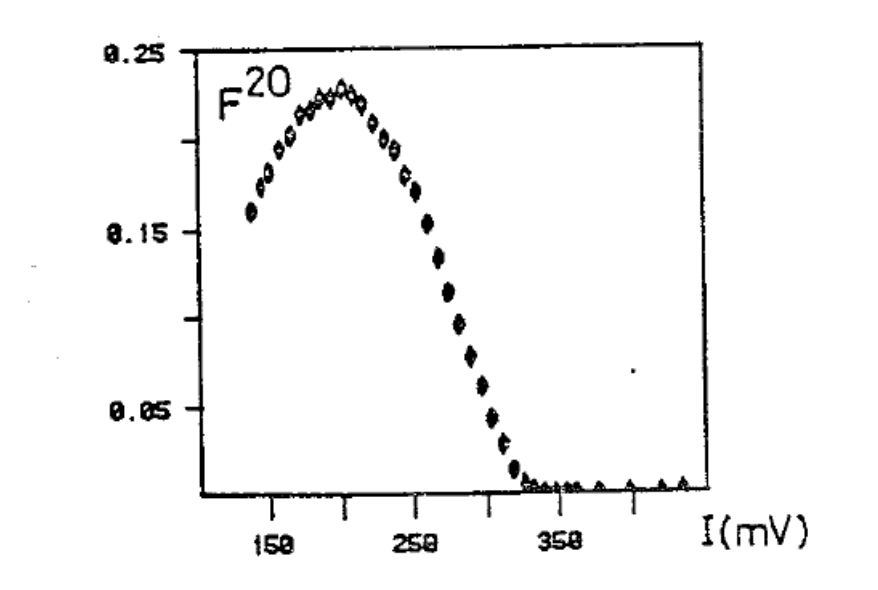
\includegraphics[width=0.78\textwidth]{fig_elmBetaSpec.png}}
	\caption{A sample beta energy spectrum using a spectrometer \cite{Elm87}.}
	\label{fig:elmspec}
\end{figure}

An important consideration is the normalization of each point.
For each spectrometer setting, the amount of measurement time, the acceptance of the spectrometer, and the source activity have to be accounted for.
To help with the normalization, a beta telescope near the target was used.
This measures the activity of the source, and takes into account the degradation of the target.
However, there are still issues with adjusting for the efficiency of the beta telescope.
This efficiency changes as the spectrometer's field is changed.
The location of the telescope was optimized to minimize this effect.
Another way of normalization was to continuously adjust the spectrometer field so that a the entire energy range is sampled over each measurement cycle.
The issue there is that changing the magnetic fields induces currents that are hard to correct for. 
In that measurement, adjusting the spectrometer field was used as a benchmark for the beta telescope normalization method.

An issue with this measurement is that the shape factor is not just the linear term.
The shape factor depend on the other nuclear form factors and are not independent.
The other terms were calculated and fixed.
Ultimately the resulting measurement of the linear term matched the CVC prediction.

Using a single detector would take care of the normalization automatically. 
A shape measurement of $^{20}$F was made with a spectrometer and a high purity germanium detector \cite{Het89}.
The linear term in the shape factor was measured just like in the previous measurement.
The magnetic field was used to enhance the solid angle for the electrons compared to the gamma rays.
The $^{20}$F was made with a deuteron beam on a natural LiF target. 
An implant and decay cycle was used to measure the beta decay spectrum. 
A calibration beta spectrum is shown in figure \ref{fig:hethspec}.

\begin{figure}[!htb]
	\begin{minipage}[b][][b]{0.50\textwidth}
		\centerline{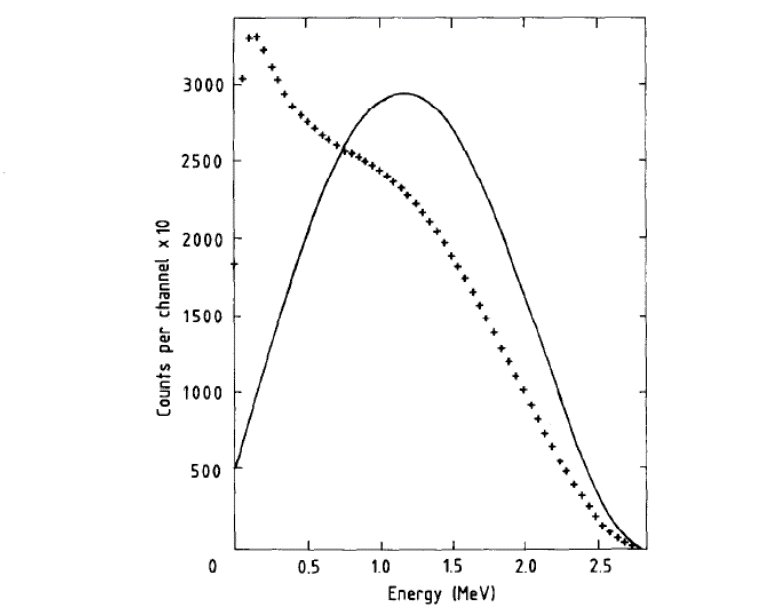
\includegraphics[width=0.9\textwidth,height = 5.33 cm]{fig_hethBetaSpec.png}}
	\end{minipage}\hfill
	\begin{minipage}[b][][b]{0.50\textwidth}
		\centerline{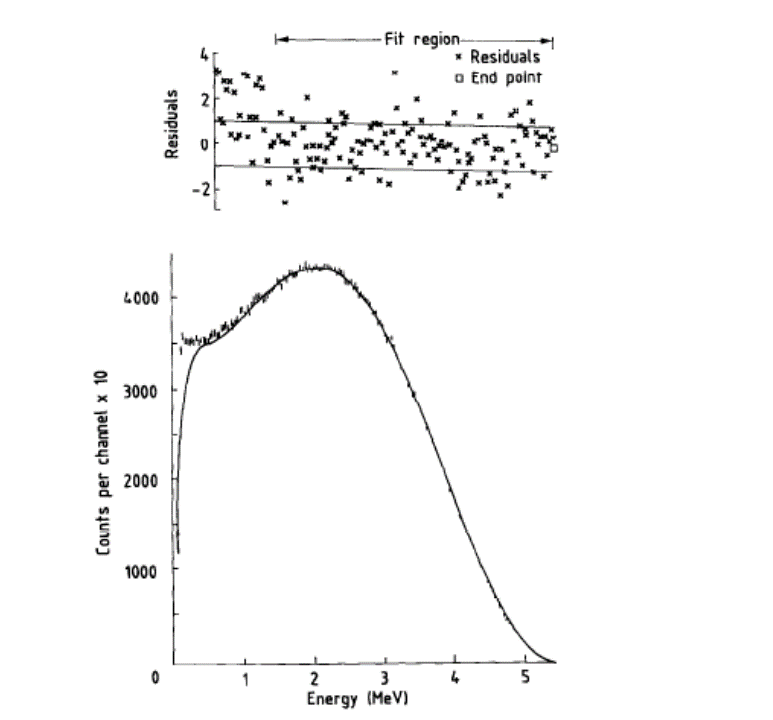
\includegraphics[width=0.9\textwidth,height = 8 cm]{fig_heth20f.png}}
	\end{minipage}
	\caption{On the left there are simulated spectra of beta spectrum measured with a scintillator \cite{Het89}.
		 The line is the original beta spectrum, and the crosses a simulated spectrum showing the back-scattering.
		 On the right is the measured and fit $^{20}$F beta spectrum.}
	\label{fig:hethspec}
\end{figure}

As seen from figure \ref{fig:hethspec}, there is a large distortion at low energies.
This is due to back-scattering inside the germanium detector.
Another issue for this measurement was that energy calibration was non-linear.
Below 1.5 MeV, there was a non-linearity which caused a distortion down to 35 keV. 
This all had to be accounted for and contributed to the uncertainty.
The resulting energy spectrum and fit is shown on the right in figure \ref{fig:hethspec}.


The beta spectrum is greatly distorted.
The effective shape measurement analysis was started at 1.5 MeV.
For this measurement there were several systematic effects.
The largest uncertainty was due to the response function.
The paper refers this to ``peak position.'' 
This experiment used many different sources to get a calibration.
They also had to take the bremsstrahlung of the electrons into account.
That systematic effect was the limiting factor in their measurement.

Much like the spectrometer measurement, the other terms of the shape factor were fixed.
Here however the other terms were calculated as a systematic error.
It was found that the $E^{2}$ term had more of an effect in the measurement than the $1/E$ term.
Ultimately, the measured linear term was consistent with the CVC hypothesis. 
%Spectrum is on page 168 in thesis. Put it here

The current work is also a spectrum shape measurement, much like the two cited above.
The ultimate goal is however a  determination of the Fierz term. 
In order to get the Fierz term, the beta energy spectrum must be described precisely.

\end{document}
